\documentclass[titlepage, a4paper]{article}
%importerat (2017-01-24) layout-bibliotek från Hannes Snögren, KMM 14/15. Med godkännande från honom. 
%ändrat i settings sedan dess. babel-bibliotek för swedish krävs för kompilering.
%debian: sudo apt-get install texlive-lang-european

\usepackage[swedish]{babel}
\usepackage[utf8]{inputenc}
\usepackage{color}
\usepackage{graphicx}
\usepackage{etoolbox}
\usepackage{hyperref}
\usepackage{calc}  
\usepackage{enumitem}
\usepackage{titlesec}

\makeatletter
\patchcmd{\ttlh@hang}{\parindent\z@}{\parindent\z@\leavevmode}{}{}
\patchcmd{\ttlh@hang}{\noindent}{}{}{}
\makeatother

%Spacing för sections och subsections
\titlespacing*{\section}
{0pt}{5.5ex plus 1ex minus .2ex}{1.0ex plus .2ex}
%\titlespacing*{\subsection}
%{0pt}{5.5ex plus 1ex minus .2ex}{4.3ex plus .2ex}

% Sidformat
\usepackage{a4wide}

% Fixa Appendix-titlar
\usepackage[titletoc,title]{appendix}

% Bättre tabeller
\usepackage{tabularx}

% Bättre bildtexter
\usepackage[margin=10pt,font=small,labelfont=bf,labelsep=endash]{caption}

% Enkelt kommando som låter mig attgöra-markera text
\newcommand{\todo}[1] {\textbf{\textcolor{red}{#1}}}

% Nytt \paragraph låter oss ha onumrerade bitar
\makeatletter
\renewcommand\paragraph{\@startsection{paragraph}{4}{\z@}%
{-3.25ex\@plus -1ex \@minus -.2ex}%
{1.5ex \@plus .2ex}%
{\normalfont\normalsize\bfseries}}
\makeatother

\providecommand{\LAYOUTlogga}{../mall/Logga.png}
\providecommand{\LAYOUTdatum}{\today}


%% Headers och Footers
\usepackage{fancyhdr}
\pagestyle{fancy}
\lhead{\includegraphics[scale=0.12]{\LAYOUTlogga}}
\setlength{\headsep}{0.4in}
\rhead{\ifdef{\LAYOUTutfardare}{Utfärdat av \LAYOUTutfardare \\\LAYOUTdatum}\LAYOUTdatum}
\lfoot{\LAYOUTkursnamn \\ \LAYOUTdokumenttyp}
\cfoot{\thepage}
\rfoot{\LAYOUTprojektgrupp \\ \LAYOUTprojektnamn}

%% Titelsida
\newcommand{\LAYOUTtitelsida}{%
{\ }\vspace{45mm}
\begin{center}
  \textbf{\Huge \LAYOUTdokument}
\end{center}
\begin{center}
  {\Large Redaktör: \LAYOUTredaktor}
\end{center}
\begin{center}
  {\Large \textbf{Version \LAYOUTversion}}
\end{center}
\vspace{5mm}
\ifdef{\LAYOUTfrontpicture}{
\begin{center}
    \LAYOUTfrontpicture
\end{center}
}

\newpage
}


% Projektidentitet
\newenvironment{LAYOUTprojektidentitet}{%
{\ }\vspace{45mm}
\begin{center}
  {\Large PROJEKTIDENTITET}\\[0.5ex]
  {\small
  \LAYOUTartaltermin, \LAYOUTprojektgrupp\\
  Linköpings Tekniska Högskola, IDA
  }
\end{center}
\begin{center}
  {\normalsize Gruppdeltagare}\\
  \def\arraystretch{1.5}%
  \begin{tabular}{|l|l|p{25mm}|l|}
    \hline
    \textbf{Namn} & \textbf{Ansvar} & \textbf{Telefon} & \textbf{E-post} \\
    \hline
}%
{%
    \hline
  \end{tabular}
\end{center}
\begin{center}
  {\small
    \ifdef{\LAYOUTgruppadress}{\textbf{E-postlista för hela gruppen}: \LAYOUTgruppadress\\}{}
    \ifdef{\LAYOUTgrupphemsida}{\textbf{Hemsida}: \LAYOUTgrupphemsida\\[1ex]}{}
    \ifdef{\LAYOUTkund}{\textbf{Kund}: \LAYOUTkund\\}{}
    \ifdef{\LAYOUTkundkontakt}{\textbf{Kontaktperson hos kund}: \LAYOUTkundkontakt\\}{}
    \ifdef{\LAYOUTkursansvarig}{\textbf{Kursansvarig}: \LAYOUTkursansvarig\\}{}
    \ifdef{\LAYOUThandledare}{\textbf{Handledare}: \LAYOUThandledare\\}{}
  }
\end{center}
\newpage
}
\newcommand{\LAYOUTgruppmedlem}[4]{\hline {#1} & {#2} & {#3} & {#4} \\}

%% Dokumenthistorik
\newenvironment{LAYOUTdokumenthistorik}{%
\begin{center}
  Dokumenthistorik\\[1ex]
  %\begin{small}
  \def\arraystretch{1.5}%
    \begin{tabular}{|l|l|p{45mm}|p{30mm}|l|}
      \hline
      \textbf{Version} & \textbf{Datum} & \textbf{Utförda förändringar} & \textbf{Utförda av} & \textbf{Granskad} \\
      }%
    {%
			\hline
    \end{tabular}
  %\end{small}
\end{center}
}

\newcommand{\LAYOUTversionsinfo}[5]{\hline {#1} & {#2} & {#3} & {#4} & {#5} \\}

% Kravlistor
\newenvironment{LAYOUTkravlista}{
	\center
		\tabularx{\textwidth}{| p{1.2cm} | p{1.9cm} | X | c |}
			\hline
			\textbf{Krav} & \textbf{Förändring} & \textbf{Beskrivning} & \textbf{Prioritet} \\\hline
}
{
		\endtabularx
	\endcenter
}

\newcounter{LAYOUTkravnummer}
\addtocounter{LAYOUTkravnummer}{1}
\newcommand{\LAYOUTkrav}[4][Krav \arabic{LAYOUTkravnummer}]{{#1} & {#2} & {#3} & {#4} \stepcounter{LAYOUTkravnummer}\\\hline}

% Milstolps-lista
\newenvironment{LAYOUTmilstolpar}{
	\center
		\tabularx{\textwidth}{| p{1.2cm} | X | l |}
			\hline
			\textbf{Nr} & \textbf{Beskrivning} & \textbf{Datum} \\\hline
}
{
		\endtabularx
	\endcenter
}

\newcounter{LAYOUTstolpnummer}
\addtocounter{LAYOUTstolpnummer}{1}
%\newcommand{\LAYOUTmilstolpe}[3][Krav \arabic{LAYOUTstolpnummer}]{{#1} & {#2} & {#3} \stepcounter{LAYOUTstolpnummer}\\\hline}
\newcommand{\LAYOUTmilstolpe}[3]{{#1} & {#2} & {#3} \\\hline}

% Aktivitets-lista
\newenvironment{LAYOUTaktivitetslista}{
	\center
		\tabularx{\textwidth}{| p{0.3cm} | X | c | c |}
			\hline
			\textbf{Nr} & \textbf{Beskrivning} & \textbf{Beroende av} & \textbf{Timmar} \\\hline
}
{
		\endtabularx
	\endcenter
}

\newcounter{LAYOUTaktivitetsnummer}
\addtocounter{LAYOUTaktivitetsnummer}{1}
% \newcommand{\LAYOUTaktivitet}[4][\arabic{LAYOUTstolpnummer}]{{#1} & {#2} & {#3} & {#4} \stepcounter{LAYOUTstolpnummer}\\\hline}
\newcommand{\LAYOUTaktivitet}[4]{{#1} & {#2} & {#3} & {#4} \\\hline}

% Mall för mötesprotokoll
\newenvironment{projektmote}[2]{
  {\ }\vspace{5mm}

  \centerline{\textbf{\Huge #1}}
  \vspace{2mm}
  \centerline{\LARGE #2}
  \vspace{10mm}

  \begin{itemize}
}
{
  \end{itemize}
}

\newcounter{paragrafnummer}
\addtocounter{paragrafnummer}{1}
\newcommand{\paragraf}[1]{\item{\textsection \arabic{paragrafnummer}. {#1}}\addtocounter{paragrafnummer}{1}}

% Mall för Statusrapport
\newenvironment{statusrapport}{
  \center
    \tabularx{\textwidth}{| p{0.4cm} | X | X | p{14.5mm} | p{13.5mm} | p{16.5mm} | p{16.5mm} |}
    \hline
    \textbf{Nr} & \textbf{Aktivitet} & \textbf{Beroenden} & \textbf{Planerad tid} & \textbf{Nedlagd tid} & \textbf{Planerad klar} & \textbf{Beräknat klart} \\\hline
}
{
    \endtabularx
  \endcenter
}

\newcommand{\aktivitetstatus}[7]{{#1} & {#2} & {#3} & {#4} & {#5} & {#6} & {#7} \\\hline}


%parametrar som behövs för layout
\newcommand{\LAYOUTredaktor}{Johan Nåtoft}
\newcommand{\LAYOUTversion}{1.1}
\newcommand{\LAYOUTdokument}{Projektplan}
\newcommand{\LAYOUTdokumenttyp}{Projektplan}
\newcommand{\LAYOUTgranskatdatum}{}
\newcommand{\LAYOUTgranskare}{}
\newcommand{\LAYOUTgodkannare}{}
\newcommand{\LAYOUTgodkantdatum}{}
\newcommand{\LAYOUTkursnamn}{TDDD96}
\newcommand{\LAYOUTprojektnamn}{Visualization}
\newcommand{\LAYOUTprojektgrupp}{Grupp 2}
\newcommand{\LAYOUTartaltermin}{VT 2017}
\newcommand{\LAYOUTgrupphemsida}{https://gitlab.ida.liu.se/tddd96/visualization}
\newcommand{\LAYOUTkund}{Kristian Sandahl}
\newcommand{\LAYOUTkundkontakt}{Kristian Sandahl}
\newcommand{\LAYOUTkursansvarig}{Kristian Sandahl}
\newcommand{\LAYOUThandledare}{Lena Buffoni}

%override paket för detta doc.
\usepackage[swedish]{babel}
\usepackage{tabularx}
\usepackage{pdfpages}
\usepackage{tikz}
\usepackage{biblatex}
\addbibresource{../mall/references.bib}

\usetikzlibrary{shapes, arrows}
\graphicspath{ {../../images/} }

\pagenumbering{roman}

\DeclareGraphicsRule{.0.pdf}{pdf}{*}{}

\begin{document}
\LAYOUTtitelsida

\begin{LAYOUTprojektidentitet}
\LAYOUTgruppmedlem{Johan Nåtoft}{Teamledare}{070-7661443}{johna702@student.liu.se}
\LAYOUTgruppmedlem{Joakim Argillander}{Testledare}{076-8618641}{joaar286@student.liu.se}
\LAYOUTgruppmedlem{Victor Bodin}{Kvalitetssamordnare}{073-5183199}{vicbo282@student.liu.se}
\LAYOUTgruppmedlem{Sebastian Callh}{Utvecklingsledare}{073-8204664}{sebca553@student.liu.se}
\LAYOUTgruppmedlem{Rebecca Lindblom}{Analysansvarig}{073-4364079}{rebli156@student.liu.se}
\LAYOUTgruppmedlem{Johan Thornström}{Arkitekt}{070-5297445}{johth918@student.liu.se}
\LAYOUTgruppmedlem{Jonathan Wahlund}{Konfigurationsansvarig}{070-6106911}{johwa732@student.liu.se}
\LAYOUTgruppmedlem{Daniel Wassing}{Dokumentansvarig}{076-7741110}{danwa223@student.liu.se}
% lägg till fler här
\end{LAYOUTprojektidentitet}

\newpage
\tableofcontents	%Innehållsförteckning
\bigskip
\textbf{Appendix A - Vår anpassning av Scrum}
\newpage

\begin{LAYOUTdokumenthistorik}
\LAYOUTversionsinfo{0.1}{2017-01-25}{Första utkast}{Daniel Wassing}{}
\LAYOUTversionsinfo{0.2}{2017-02-06}{Dokumentplan, Resursplan, Tidsram}{Daniel Wassing}{}
\LAYOUTversionsinfo{0.3}{2017-02-07}{Fler subdokument}{Daniel Wassing}{}
\LAYOUTversionsinfo{1.0}{2017-02-20}{Första version för inlämning 1}{Daniel Wassing}{}
\LAYOUTversionsinfo{1.1}{2017-03-20}{Revidering efter opponering}{Daniel Wassing}{}
\end{LAYOUTdokumenthistorik}

\newpage
\pagenumbering{arabic} %Påbörja sidnumrering

%inputs go here
% Ordlista ska ej med i innehållsförteckningen
\section*{Ordlista}
Här följer förklaring av förkortningar som används genom hela detta dokument.
\begin{description}[leftmargin=!,labelwidth=\widthof{\bfseries Some text}]
\item[CI] Continous Integration
\item[IDA] Institutionen för Datateknik vid Linköpings Universitet
\end{description}
\newpage
\section{Introduktion}
Följande dokument utgör en kravspecifikation för projektet. 
\subsection{Syfte och målgrupp}
Syftet med kravspecifikationen är att tydliggöra alla projektets intressenters krav på applikationen. Kravspecifikationen utgör ett konstruktionsunderlag såväl som underlag för dokumentation och testning av applikationen. Kravspecifikationen ska användas som beslutsunderlag för när beslut ska tas om projektet.
\\
\\
Målgruppen för dokumentet är alla projektets intressenter, däribland beställare, utvecklare och testare. 
\subsection{Avgränsningar}
Applikationen är ett verktyg för visualisering och utför således ingen databehandling. Den behöver heller inte fungera på mindre skärmar och handhållna enheter eller stödja andra språk än engelska.

\begin{table}[h!]
  \centering
  \caption{En tabell över utvecklingsplattformar.}
  \def\arraystretch{1.5}
  \begin{adjustbox}{max width=\textwidth}
    \begin{tabularx}{\textwidth}{ | l | X | }
      \hline
      \textbf{Operativsystem} & \textbf{Webbläsare} \\
      \hline
      Ubuntu 16.04 & Firefox 51.0.1 \\
      \hline
      macOS Sierra 10.12.3 & Chrome 55.0.2883.95 \\
      \hline
      Windows 8.1, 10 & Chrome 55.0.2883.95 \\
      \hline
    \end{tabularx}
  \end{adjustbox}
  \label{tab:utvecklingsplattformar}
\end{table}
\ \\
Utvecklingen och testning kommer ske på de plattformar som ses i tabell \ref{tab:utvecklingsplattformar} och applikationen är därmed inte garanterad att fungera på andra plattformar. Applikationen kommer att utvecklas som en forskningsprototyp.

\subsection{Dokumentkonventioner}
\subsubsection{Format på krav}
Kraven på produkten kommer att anges löpande i de olika avsnitten.

\begin{table}[h!]
  \centering
  \caption{En tabell över format på krav.}
  \def\arraystretch{1.5}
  \begin{adjustbox}{max width=\textwidth}
    \begin{tabularx}{\textwidth}{ | c | l | X | c | }
      \hline
      Kravnummer & Förändring & Kravtext & Prioritet \\
      \hline
    \end{tabularx}
  \end{adjustbox}
  \label{tab:krav_format}
\end{table}
\ \\
Kraven på produkten ges på följande form enligt tabell \ref{tab:krav_format}. Alla krav numreras från K1 och framåt där K indikerar att det är ett krav. Förändring indikerar om kravet är annorlunda från originalkravet. Kravtext ger information om kravet. Prioritet anger om kravet är ett baskrav som uppfylls under utvecklingsiteration 1 (prioritet 1), eller ett krav som uppfylls i en senare utvecklingsinteration (prioritet 2), eller om det är ett krav vid eventuell vidareutveckling (prioritet 3).

\newpage
\subsubsection{Definitioner}
Här följer förklaring av ord som används genom hela detta dokument.

\begin{description}[leftmargin=!,labelwidth=\widthof{\bfseries Continous Integration}]
\item[Artefakt] En faktiskt produkt, t.ex. en JavaScript-klass eller ett dokument.
\item[Commit] En uppsättning ändringar i ett versionshanteringssystem.
\item[Continous Integration] Arbetsmetodik för att kontinuerligt integrera, bygga och testa systemändringar.
\item[Chrome] Webbläsare.
\item[Eiffel] Ramverk från Ericsson som i det här projektet används för att spåra händelser i CI-system. Ramverket har länge används internt på Ericsson men blev nyligen publikt. Eiffel som helhet har inga versioner, det system som används i projektet är det som finns publicerat i commit 0303cf3. \cite{website:eiffel}
\item[Firefox] Webbläsare.
\item[Händelseförlopp] Beskriver den kedja av händelser som sker p.g.a. en ändring i ett CI-system. Kedjan initeras av en kodändring och begränsas av att en pålitlighetsgrad sätts.
\item[JavaScript] Programmeringsspråk som i projektet används för att skriva applikationen.
\item[macOS] Operativsystem.
\item[Meteor] Ramverk för webbutveckling som använder JavaScript. Version 1.4.2.6 används i detta projekt. \cite{website:meteor}
\item[Pålitlighetsgrad] Mått på hur väl en artefakt presterat vid testning.
\item[README-fil] Fil med information om en applikation, t.ex. hur den används eller systemkrav.
\item[Repository, repo] Lagringsutrymme för versionshanterade artefakter.
\item[Ubuntu] Operativsystem.
\item[Windows] Operativsystem.
\end{description}

\subsection{Översikt}
Kravspecifikationen innehåller en beskrivning av produkten där en tolkning av kundkraven har gjorts och dess funktioner och användaregenskaper beskrivs. Kravspecifikationen innehåller också de specifika krav som formulerats utifrån den tolkning som gjorts av kundens krav och önskemål beträffande gränssnitt, funktioner och prestandakrav samt begränsningar. %fluff
\newpage
\section{Begränsningar}
Projektets resurs är specificerad i tid och således består dess begränsningar av det.
\subsection{Tid}
Projektets tidsbegränsning innefattas av kursen TDDD96, 15 högeskolepoäng. Tidsbegränsningen är 400 timmar ,$\pm$ 10\%, per gruppmedlem och 3200 timmar för hela gruppen. De 400:a timmarna sträcker sig till och med projektets avslut, specificerat under kapitel 5.2 Beslutspunkter. Då beräknas den veckovisa tidsbudgeten till ca 20 timmar med lite förändringar beroende på hur mycket tid som lagts tidigare veckor.Tidsbudgeten har undantag för tentaperioder då arbete är frivilligt men uppskattas. 
\subsection{Budget}
Projektets budget är specificerad i tid. Inga övriga begränsningar finns för projektet.  %budget, tid osv
\newpage
\section{Projektmål}
Applikationen är ett verktyg för att tydligt få en överblick över händelser och flöden i CI-processer för ett system, exempelvis byggen och tester. Applikationens målgrupp är företag som bedriver mjukvaruutveckling med större utvecklingsteam. Företaget använder sig i dagsläget av CI och vill kunna upptäcka flaskhalsar och förbättra sitt arbetsflöde. Applikationen är en webbaserad tjänst som kommer att skrivas i JavaScript. Data som visualiseras i applikationen kommer från valfritt CI-system, och generaliseras med hjälp av ramverket Eiffel. Händelser och flöden visualiseras genom interaktiva grafer där användaren kan välja att visa data i flera olika nivåer för att kunna dra slutsatser sitt utvecklingsflöde. 
\\
För mer detaljerad information se kravspecificationen.

\iffalse
\begin{figure}[h]
    \centering
    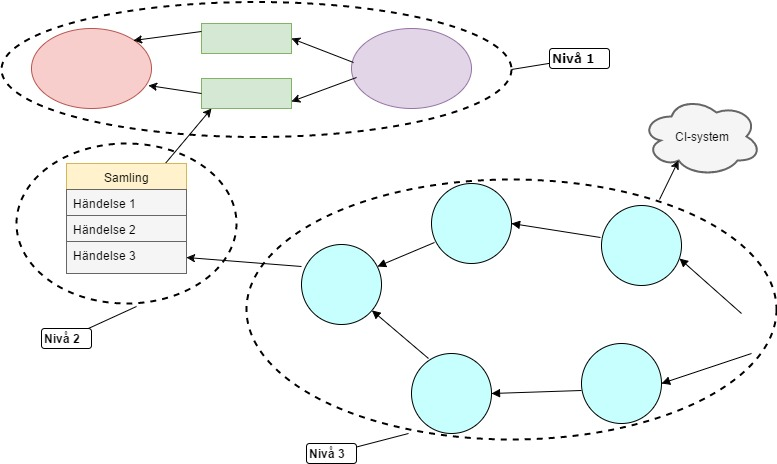
\includegraphics[width=\textwidth]{Visualization}
    \caption{De olika nivåerna av systemet, godtyckligt färgade.}
    \label{fig:system_overview}
\end{figure}
\fi

\subsection{Affärsmål}
Applikationen ska visualisera händelser i ett CI-system så att en beslutsfattande person som inte har kunskaper inom programmering ska kunna fatta beslut hur resurser ska fördelas.

\subsection{Systemmål}
För systemmål se arkitekturdokumentet.

\subsection{Kvalitetsmål}
För kvalitetsmål se kvalitetplanen.
 %mål med projektet
\newpage
\section{Resursplan}
För att kunna planera projektet har en resursplan över projektets leverabler och aktiviteter tagits fram. Här återfinns de beslutspunkter och milstolpar som projektgruppen förhåller sig till.
\subsection{Beslutspunkter} %tollgates

	Alla datum avser år 2017.\\
	\\
	\begin{tabular}{l l}
	23/1: &	Tilldelning av projekt \\
	1/2:  & Deadline för avtal med kund \\
	15/2: & Pitch-Seminarium \\
	20/2: & Inlämmning av iteration 1 \\
	8/3:  & Inlämmning av iteration 2 \\
	24/4: & Inlämmning av iteration 3 \\
	8/5:  & Inlämmning av kandidatrapport \\
	24/5: & Slutseminarium \\
	29/5: & Slutversion till Kristian Sandahl \\
	\end{tabular}	


\subsection{Resurser}%vet inte om det nämns på fler ställen
Projektruppen innehåller 8 st personer med 400 timmar budgeterat per person. Gruppen har även en handledare att tillgå som resurs. Förutom de tilldelade resurserna finns datorsalar att tillgå på IDA och lokaler på Linköpings universitet. Kunden har möjlighet att tillhandahålla virtuell maskin som server under utveckling av produkten. Resurser som finns inom gruppen tas till vara på, om någon är mer erfaren inom ett område så delas den med sig av under ett utbildningstillfälle eller vid förfrågan om hjälp.\\
\newpage %milstolpar, krav-grindar, delresultat, aktiviteter, resurser
\newpage
\section{Fasplan}
Projektet utförs i iterationer enligt vår scrum-modell (se stycke 6.6, scrum). Varje iteration är 2 veckor lång.

\subsection{Förstudie}
Under förstudien skall projektplan, kravspecifikation, kvalitetsplan, statusrapport och systemanatomi skrivas. Dokument som ska vara påbörjade men inte behöver vara färdiga är arkitekturdokument och testplan.

\subsection{Iterationer}
Under iterationerna kommer vi jobba med prio 1 kraven tills alla är uppfyllda. Om vi har tid kvar när alla krav av prioritet 1 är uppfyllda så kommer vi fortsätta arbeta med prioritet-2-kraven.

%Iteration 3 är den sista övergripande fasen av projektet. När kunden anser att kraven har blivit tillräckligt uppfyllda anses projektet avklarat. Därefter skall systemet levereras tillsammans med teknisk dokumentation och användarhandledning. Slutlig dokumentation ska skrivas och revideras. En slutrapport skall skrivas. All dokumentation skall lämnas in.

%Under iteration 2 så skall projektet genomföras. Det ska konstrueras och testas enligt kravspecifikationen, kvalitetsplanen, arkitekturdokumentet och testplanen. Det skall även skrivas teknisk dokumentation och en användarhandledning ska påbörjas. %iterationer som subsections?
\newpage
\section{Organisationsplan för projektet}
Här presenteras projektets organisation.

\subsection{Roller}
De olika roller som projektgruppen valde att arbeta i var:\\
\begin{itemize}
\item Teamledare - Johan Nåtoft
	\begin{itemize}
		\item Teamledarens roll är att se till att projektets mål uppfylls. Det är även dennes ansvar att vara projektgruppens ansikte utåt och sköta all kontakt med projektledningen. Teamledaren är också en coach till medlemmarna i projektet och ska agera bollplank samt ska se till att gruppen har ett gott samarbete sinsemellan. 
	\end{itemize}
\item Konfigurationsansvarig - Jonathan Wahlund
	\begin{itemize}
		\item Bestämmer vilka produkter som skall versionshanteras samt vilka arbetsprodukter som skall ingå i en utgåva. Ser till att verktygen som används för versionshantering används på rätt sätt och att dessa är underhållna. Är även ansvarig för att hitta lösningar till problem som gruppen kan stöta på med verktygen. 
	\end{itemize}
\item Testledare - Joakim Argillander
	\begin{itemize}
		\item Beslutar om systemets status och ansvarar för att en testplan samt testrapport skrivs. Ansvarig för att tester utformas enligt rådande och överenskommen standard. Ansvarig för att kravspecifikationen är testbar och att testfall körs för alla testbara krav. Delegerar testuppgifter och sätter upp en testplan i mån av uppgifter och tidsplan för denna.
	\end{itemize}
\item Kvalitetsansvarig - Victor Bodin
	\begin{itemize}
		\item Ansvarig för att sammanställa en kvalitetsplan, samla in erfarenheter från gruppens medlemmar och dokumentera dessa. Planerar även för eventuell utbildning och inspiration för gruppen. Samarbetar med samtliga av gruppens medlemmar för att nå en hög nivå av kvalitet genom hela projektet. Ser även till att följa upp på de aktiviteter som vi beslutar om så att vi vet vad som kan göras bättre eller tydliggöra vad vi gjorde för fel.
	\end{itemize}
\item Utvecklingsledare - Sebastian Callh
	\begin{itemize}
		\item Ansvarig för fördelningen av utvecklingsarbetet och den detaljerade designen på systemet. Gör beslut angående utvecklingsmiljö och är även Scrum-master, där uppgifter så som att organisera utvecklingsarbetet och bistå med teknisk kompetens ingår.
	\end{itemize}
\item Arkitekt - Johan Thornström
	\begin{itemize}
		\item Ansvarig för att ta fram en arkitektur och identifiera komponenter samt gränssnitt. Gör även de övergripande teknikvalen och har även mest inflytande i tekniska frågor. Samrådar med utvecklingsledaren hur tekniska frågor ska tacklas och ansvarar för att gränssnitt finns och följs.
	\end{itemize}
\item Analysansvarig - Rebecca Lindblom
	\begin{itemize}
		\item Denna person sköter kontakten med kund och är även direkt ansvarig för kraven som ställs på projektet samt för att dokumentera dessa. Analysansvarig ansvarar även för att kravspecifikationen blir skriven även om personen inte är ensam om att skriva den.
	\end{itemize}
\bigskip
\item Dokumentansvarig - Daniel Wassing
	\begin{itemize}
		\item Ansvarig för skapandet av dokumentmallar och struktur. Även ansvarig för projektetslogga samt har en övergripande koll på deadlines för olika dokument. Är även ansvarig för att dokumentera på möten som hålls och att revidera dessa så att de är tydliga och användbara.
	\end{itemize}
\end{itemize}

\subsection{Kunskap}
Projektgruppens kunskap är varierande och bred. Gruppen ska jobba kontinuerligt för att dela med sig av nödvändig kunskap till samtliga medlemmar.
Den kunskap som förväntas att finnas hos gruppmedlemmarna är de förkunskapskrav som ställs på alla studenter som gör kandidatarbetet.

\subsection{Utbildning}
Projektgruppen kommer ta del av interna utbildningar inom testning, Git och JavaScript i största möjliga mån och vid behov. Vi värdesätter att vår kod är bra så vi har haft en utbildning inom testbar kod.
\begin{itemize}
\item Powerpoint slides för testbar kod - \url{https://goo.gl/oUiBwL}
%lägg till mer utbildningsgrejer här
\end{itemize}

\subsection{Kommunikation}
All kommunikation inom gruppen som inte sker fysiskt sker genom verktyget Slack. Kommunikation med kunden går genom teamledaren och analysansvarig via mail.

\subsection{Rapporter}
Intern dokumentering och organisation sker på Google Drive medan alla officiella dokument produceras i LaTeX och versionhanteras genom Git. I tabell \ref{tab:dokumentation} nämns alla officiella dokument som kommer produceras under projektets gång. Alla gruppmedlemmar rapporterar den tid de arbetat med projektrelaterade uppgifter i ett rapporterings-dokument på Google Drive. 

\subsection{Agil arbetsmetodik}
Projektets utveckling kommer att bedrivas enligt Scrum, med diverse modifikationer för att fungera tillsammans med gruppens övriga studier. En jämförelse mellan renordnad Scrum och vår tillämpning av det finns i appendix A. %roller, kunskap/färdigheter, utbildning, kommunikation och rapporter
\newpage
\section{Dokumentplan}
Dokumentation listad i tabell \ref{tab:dokumentation} ska utföras.

\begin{table}[h]
\centering
\caption{Dokumentation.}
\def\arraystretch{1.5}%
\begin{tabularx}{\textwidth}{| p{20mm} | X | X | X | X | X |}
	\hline
	\textbf{Dokument} & \textbf{Ansvarig} & \textbf{Godkänns av} & \textbf{Syfte} & \textbf{Distribu- eras till} & \textbf{Färdig datum} \\\hline
	{Projektplan} & {Johan Nåtoft} & {Kristian Sandahl} & {Plan för hur projektet ska utföras} & {Kristian Sandahl} & {} \\\hline
	{Kravspeci- fikation} & {Rebecca Lindblom} & {Kristian Sandahl} & {Krav som ska uppnås under projektets gång} & {Kristian Sandahl} & {} \\\hline
	{Kvalitetsplan} & {Victor Bodin} & {Kristian Sandahl} & {Hypotes om hur arbetet ska fungera} & {Kristian Sandahl} & {} \\\hline
	{Statusrapport} & {Johan Nåtoft} & {Kristian Sandahl} & {Information om huruvida vi har nått målen med förstudien} & {Kristian Sandahl} & {} \\\hline
	{Systemana- tomi} & {Johan Nåtoft} & {Kristian Sandahl} & {En visualisation av projektets anatomi} & {Kristian Sandahl} & {} \\\hline
	{Arkitektur- dokument} & {Johan Thornström} & {Kristian Sandahl} & {Dokument för struktur av projektet} & {Kristian Sandahl} & {} \\\hline
	{Testplan} & {Joakim Argillander} & {Kristian Sandahl} & {Plan för hur testning ska genomföras} & {Kristian Sandahl} & {} \\\hline
	
\end{tabularx}
\label{tab:dokumentation}
\end{table}
\newpage

\newpage
\section{Mötesplan}
Utöver planerade veckomöten så hålls även extramöten vid behov. Under varje möte så skapar vi ett nytt mötesprotokoll utifrån vår protokoll-mall. Mötena sker internt i gruppen och i vissa fall även med handledare närvarande. Inför mötena ska gruppmedlemmar ha fört in punkter i dagordningen, detta för att få en bättre struktur på mötet när det väl är igång.
\subsection{Veckomöten}
Varje vecka så har vi ett oblikatoriskt veckomöte där vi går igenom vad vi har gjort under senaste veckan och vad vi ska göra under kommande vecka.
\subsection{Handledarmöten}
Handledarmötena sker tillsammans med handledare Lena Buffoni en gång per vecka. De mötena är en avstämning utifrån genomförande och planeringssynvinkel.\\ \\
Mötena kan ha två olika upplägg beroende på vad projektgruppen tycker känns relevant. Antingen håller projektgruppen ett eget möte med handledaren som observatör och kommer med kommentarer. Eller så håller hon i mötet utifrån mötespunkter som projektgruppen satt upp i förväg och meddelat handledaren.
\subsection{Kundmöten}
I projektets början används kundmötena för att reda ut projektets krav och vad applikationen förväntas innehålla. Senare i projektet används kundmötena för att stämma av hur utvecklingen går samt se att projektet går i rätt riktning. Kundmötena planeras in när kunden eller projektgruppen känner att behovet finns. Vid kundemötena representeras projektgruppen av teamledare och analysansvarig. %kanske kan vara subsection till organisationsplanen
\newpage
\section{Riskhantering}
En plan med utförlig beskrivning och förslag på risker och hur riskhantering ska gå till finns att läsa under rubriken Riskhantering i dokmentet Projektplan.
\newpage
\section*{Appendix A - Vår anpassning av Scrum}
Nedan följer en definition av den Scrumversion som gruppen arbetar utifrån.

\subsection*{Anpassning av Scrum}
Det här dokumentet syftat till att specificera de anpassningar som gruppen gör jämfört med “renodlad” Scrum. Det är skrivet innan utvecklingen börjat och kommer tjäna som utgångspunkt för framtida ändringar och förbättringar.
\subsection*{Sprinter}
I scrum är arbetet strukturerat i två-fyra veckor långa sprinter. I vår tillämpning kommer vi använda oss av två veckor långa sprinter.
\subsection*{Scrummöten}
I scrum håller scrummästaren dagliga scrummöten där teamet går igenom vad de gjort sedan gårdagen, vad de skall åstadkomma under dagen och vilka problem som förutses. På grund av att gruppen ej arbetar på heltid med projektet och har olika kurser parallellt är schemakrockar en verklighet och möten kommer hållas veckovis istället för dagligen.
\subsection*{Produktägaren}
I scrum agerar produktägaren som representant för kunden och det är dennes uppgift att leverera prioriterade user stories till utvecklingsteamet. Det kräver stor kunskap hos en enskild person för att kunna ta fram korrekta user stories och prioritera dem rätt, vilket inte kan förväntas av en grupp som prövar scrum för första gången utan någon utbildning i det. På grund av det så är det hela gruppens uppgift att under mötestid arbeta fram user stories och prioritera dem korrekt. Gruppens analysansvarig kommer även att hålla i produktägarens alla kommunikativa bitar med kund.
\subsection*{Utvecklingsteamet}
Vårt utvecklingsteam består av åtta personer, vilket ligger inom Scrums rekommenderade antal på sex-nio. Det är självorganiserande och kommer organiseras av scrummästaren endast i nödfall.
\subsection*{Scrummästaren}
Gruppens scrummästare kommer agera likt Scrums definition. Denne kommer främst arbeta för att undanröja hinder för teamets utvecklingsarbete och organisera scrummöten.
\\
Källa: http://www.scrumguides.org/\cite{website:scrum_guide} 2016 update



%... add more as needed
\clearpage
\printbibliography
\begin{appendices}

\end{appendices}
\end{document}
